\documentclass{article}
\usepackage[utf8]{inputenc}

\usepackage[letterpaper,margin=1in]{geometry}

\usepackage{biblatex}
\addbibresource{abstract.bib}

\usepackage{graphicx}
\graphicspath{{./images/}}

\title{How fast did Cicero speak?}
%\author{(Author name removed)}
\date{}

\usepackage{tipa}

\begin{document}

\maketitle

\section{Introduction}

In 2019, Coupé et al demonstrated that, while rate of speech (syllables spoken per second) and information density (bits conveyed per syllable) vary significantly between languages, their product (bits conveyed per second) does not. This ``information rate'' seems to be a property of the communicative niche of human language in general, a true linguistic universal.

Using new methods for extrapolating from limited corpora, we were able to estimate the information density for Classical Latin. From this we can predict the natural rate of speech of the Romans during the classical era, and compare it against modern Romance languages.

\section{Methods}

\subsection{Preprocessing}

The first step in calculating information density involved converting the Latin text to a phonemic representation, generally following Allen's 1978 analysis. The phonemic form is almost entirely predictable from the written form, with only a few exceptions: standard Latin orthography doesn't indicate vowel length (\emph{alium} /a.li.um/ ``another'', \emph{alium} /a\textlengthmark{}.li.um/ ``garlic'') or distinguish vowels from semivowels (\emph{soluit} /so.lu.it/ ``was accustomed'', \emph{soluit} /sol.wit/ ``releases'').

Both of these exceptions, fortunately, were accounted for by Winge 2015, who built automated tools to resolve these ambiguities with over 98\% accuracy. The rest of the preprocessing involved giving every phoneme an unambiguous representation and calculating syllable breaks, using a modified version of an algorithm by Johnson. The only non-phonemic detail included, after Oh 2015, was neutralization: if the distinction between two phonemes was lost in a particular environment, that distinction was removed in preprocessing.

\subsection{Analysis}

The standard measure of information density used by Coupé, following Oh, is syllable-conditional entropy: the average amount of information conveyed by a single syllable, given knowledge of what syllable came before it. This can be estimated from a corpus by measuring the frequency of all syllables and contexts.

Previous studies mostly used corpora with tens or hundreds of millions of tokens, while the Packard Humanities Institute corpus for Latin has only 2.2 million; excluding post-Classical works like the \emph{Digesta} of Justinian reduces this even further. Thus, new methods of extrapolation were necessary to come up with usable values for the entropy.

As Oh noted, as the corpus size increases, the estimated entropy grows sharply at first, then levels off and converges. Experimentally, we determined that this growth follows a negative power function, \( a_1 - a_2 (x - a_3)^{-a_4} \); by fitting this function to the data with least squares, we can see what value the entropy would converge to if our corpus were infinitely large.

%\begin{figure}[h]
%\caption{Estimated entropy of English (red) and Latin (blue), as a function of corpus size}
%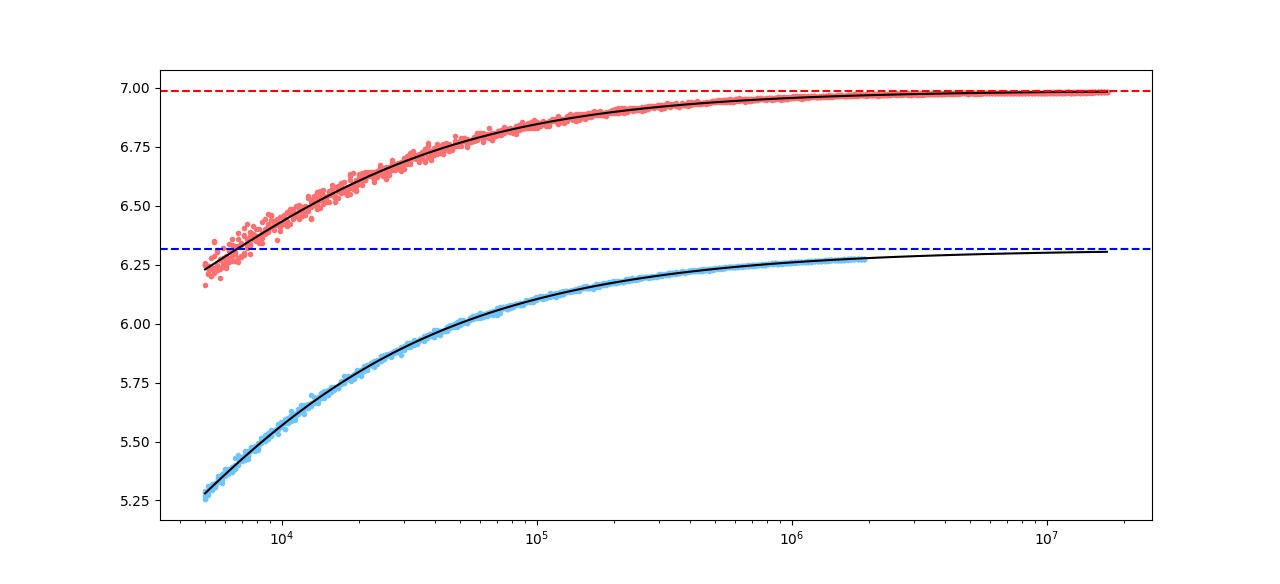
\includegraphics[width=\linewidth]{english_latin}
%\end{figure}

Even if this method allows us to extrapolate from a small corpus, though, there's still a risk that the corpus may not be representative. To test this, we used ``author jackknifing'': we gathered a list of all authors who contributed at least 100,000 tokens to the corpus, then performed the calculation with each one individually removed. The standard deviation of the results gives an approximation of how much the entropy value could be swayed by any particular author's style.

\section{Results}

In the end, we estimated a conditional entropy of 6.32 bits per syllable, with a standard error of 0.033 bits per syllable.

Coupé reports a mean information rate of 39.15 bits per second across languages, with a standard deviation of 5.10 bits per second; combining these values with our calculated entropy, we predict that Classical Latin was spoken at an average rate of 6.19 syllables per second, with a standard deviation of 0.81 syllables per second. This variance is almost entirely due to differences in speech rate within a language, with the approximation error in the entropy calculations being negligible by comparison.

\section{Conclusion}

Using new methods of extrapolation, we estimated the syllable-conditional entropy of a language from a relatively small corpus. By combining this with Coupé's proposed universal of information rate, we were able to determine the rate at which Classical Latin would have been spoken by native speakers thousands of years ago.

Notably, our results indicate that Classical Latin was spoken significantly slower than modern Romance languages---experiments have shown a mean value of 7.73 syllables per second for Spanish, for example, and 7.16 syllables per second for Italian. This makes sense from a historical perspective, as complex onsets and codas were frequently broken up or simplified in the evolution of Romance, reducing the information load carried by each individual syllable.

This suggests multiple avenues for further research. These methods could be applied fairly directly to other languages for which only written corpora exist; the primary difficulty there lies in automatically determining phonemic representations from ambiguous writing systems.

Focusing on Latin in particular, it should also be possible to calculate the effects of the various sound changes that led to modern Romance languages, and determine how much the speech rate was affected by the rearrangement of the vowel system, the breaking of initial clusters, the loss of various coda consonants, and so on. We hope to pursue these directions further.

\nocite{*}

\printbibliography

\end{document}
